\subsection{Some more difficult examples}

\begin{example}
To differentiate $$\sin\left(\sqrt{1+x^2}\right)$$ we must use the chain rule twice.

\begin{align*}
\frac{d}{dx}\left(\sin\left(\sqrt{1+x^2}\right)\right)&=\frac{d}{dx}\left(\sin\left((1+x^2)^\frac{1}{2}\right)\right)\\
&=\cos\left((1+x^2)^\frac{1}{2}\right)\cdot\frac{d}{dx}\left((1+x^2)^\frac{1}{2}\right)\\
&=\cos\left((1+x^2)^\frac{1}{2}\right)\cdot\frac{1}{2}(1+x^2)^{-\frac{1}{2}}\frac{d}{dx}\left(1+x^2\right)\\
&=\cos\left((1+x^2)^\frac{1}{2}\right)\cdot\frac{1}{2}(1+x^2)^{-\frac{1}{2}}\cdot2x\\
&=\frac{x\cos\left(\sqrt{1+x^2}\right)}{\sqrt{1+x^2}}
\end{align*}

\end{example}

\begin{example}
To differentiate $$(x^2+3)\sin x\cos x$$ we must use the product rule twice.

\begin{align*}
\frac{d}{dx}\left((x^2+3)\sin x\cos x)\right)&=(x^2+3)\frac{d}{dx}\left(\sin x\cos x\right)+\sin x\cos x\frac{d}{dx}\left(x^2+3\right)\\
&=(x^2+3)\left(\sin x\frac{d}{dx}\left(\cos x\right)+\cos x\frac{d}{dx}\left(\sin x\right)\right) + 2x\sin x\cos x\\
&=(x^2+3)\left(-\sin^2 x+\cos^2 x\right) + 2x\sin x\cos x\\
\end{align*}

\end{example}

\begin{example}
To differentiate $$\sqrt{x^2-3}\sin x$$ we must use the product rule and the chain rule.

\begin{align*}
\frac{d}{dx}\left(\sqrt{x^2-3}\sin x\right)&=\frac{d}{dx}\left((x^2-3)^\frac{1}{2}\sin x\right)\\
&=\sin x\frac{d}{dx}\left((x^2-3)^\frac{1}{2}\right)+(x^2-3)^\frac{1}{2}\frac{d}{dx}\left(\sin x\right)\\
&=\sin x\cdot\frac{1}{2}(x^2-3)^{-\frac{1}{2}}\cdot2x+(x^2-3)^\frac{1}{2}\cos x\\
&=\frac{\sin x}{\sqrt{x^2-3}}+\sqrt{x^2-3}\cos x\\
\end{align*}

\end{example}

\begin{example}
To differentiate $$\tan x$$ we can use the product rule and the chain rule.

\begin{align*}
\frac{d}{dx}\left(\tan x\right)&=\frac{d}{dx}\left(\frac{\sin x}{\cos x}\right)\\
&=\frac{d}{dx}\left(\sin x(\cos x)^{-1}\right)\\
&=\sin x\frac{d}{dx}\left((\cos x)^{-1}\right)+(\cos x)^{-1}\frac{d}{dx}\left(\sin x\right)\\
&=\sin x\cdot-(\cos x)^{-2}\cdot-\sin x+(\cos x)^{-1}\cos x\\
&=\frac{\sin^2 x}{\cos^2 x}+\frac{\cos x}{\cos x}\\
&=\tan^2 x +1
&=\sec^2 x
\end{align*}
This is one way of showing that the derivative of $\tan x$ is $\sec^2 x$.
\end{example}

\subsection{The quotient rule}
The quotient rule is a special case of the product rule. It is up to you whether you learn and use the quotient rule or whether you use the product rule instead.
\begin{thing}{The quotient rule}
If $f$ and $g$ are differentiable, then
\[\frac{d}{dx}\left( \frac{f(x)}{g(x)} \right) = \frac{f'(x)g(x) - f(x)g'(x)}{(g(x))^2}\]
\begin{proof}
Apply the product and chain rules to $f(x)(g(x))^{-1}$
\end{proof}
\end{thing}

\begin{example}
To differentiate $$\tan x$$ we can use the quotient rule.

\begin{align*}
\frac{d}{dx}\left(\tan x\right)&=\frac{d}{dx}\left(\frac{\sin x}{\cos x}\right)\\
&=\frac{\cos x\cos x - \sin x\cdot-\sin x}{\cos^2x}\\
&=\frac{\cos^2 x + \sin^2 x}{\cos^2x}\\
&=\frac{1}{\cos^2x}\\
&=\sec^2 x
\end{align*}
This is another way of showing that the derivative of $\tan x$ is $\sec^2 x$.
\end{example}

\section{Polar co-ordinates}
The chain rule can be rearranged to give:

\begin{in_a_box}
\[\frac{dy}{dx}=\frac{dy/dt}{dx/dt}\]
\end{in_a_box}

This can be used whenever $y$ and $x$ are known in terms of a parameter $t$.

\begin{example}
If $x=t^2 + 4$ and $y=e^t$ then:
\begin{align*}
\frac{dy}{dx}&=\frac{dy/dt}{dx/dt}\\
&=\frac{e^t}{2t}\\
\end{align*}
In most cases, the answer can be left in terms of $t$.
\end{example}

This is particularly useful when a function is defined using polar co-ordinates:
\begin{example}
To find the gradient of the cardiod given by the polar equation $r=1-\cos\theta$,
we must first write $x$ and $y$ in terms of $\theta$.

\begin{figure}[H]
  \centering
  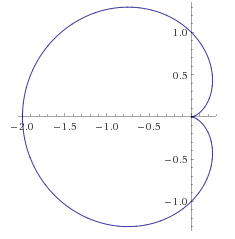
\includegraphics[scale=0.6]{img/1-costheta.png}
  \caption{The cardiod with polar equation $r=1-\cos\theta$.}
\end{figure}

\begin{align*}
x&=r\cos\theta\\
&=(1-\cos\theta)\cos\theta\\
&=\cos\theta-\cos^2\theta
\end{align*}
\begin{align*}
y&=r\sin\theta\\
&=(1-\cos\theta)\sin\theta\\
&=\sin\theta-\sin\theta\cos\theta
\end{align*}

Now we can differentiate:

\begin{align*}
\frac{dy}{dx}&=\frac{dy/d\theta}{dx/d\theta}\\
&=\frac{\cos\theta + \sin^2\theta-\cos^2\theta}{-\sin\theta+2\cos\theta\sin\theta}\\
\end{align*}
\end{example}


\section{Uses of differentiation}
\subsection{Finding the gradient at a point}
To find the gradient of a curve at a given $x$ co-ordinate, simply substitute the value of $x$ into the derivative.
\begin{example}
To find the gradient of $y(x)=x^3 - x^2$ at $x=3$, first find $y'(x)$:
$$y'(x) = 3x^2-2x$$
Next subsitute $x=3$:
\begin{align*}y'(3)&=3\cdot3^2-2\cdot3\\&=21\end{align*}
\end{example}
\subsection{Finding the maximum and minimum points}
At a point where $\frac{dy}{dx}=0$, there are three possibilites:

\begin{figure}[H]
    \hspace{0.2cm}
    \subfigure[{\it Local maximum.}]{\label{fig:local-max}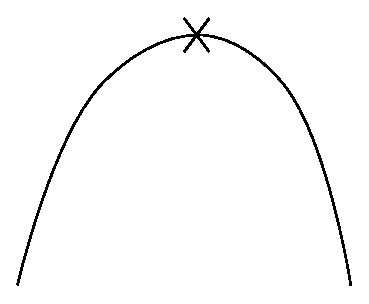
\includegraphics[scale=0.6]{img/local-max}}
    \hspace{1.5cm}
    \subfigure[{\it Point of inflection.}]{\label{fig:local-inflection}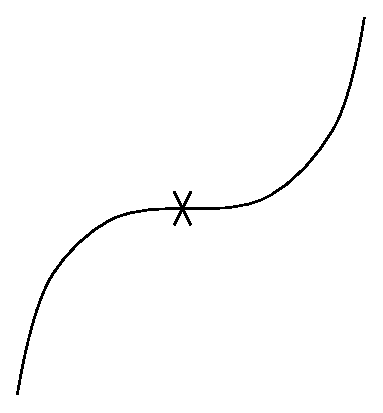
\includegraphics[scale=0.6]{img/local-inflection}}
        \hspace{1.4cm}
    \subfigure[{\it Local minimum.}]{\label{fig:local-min}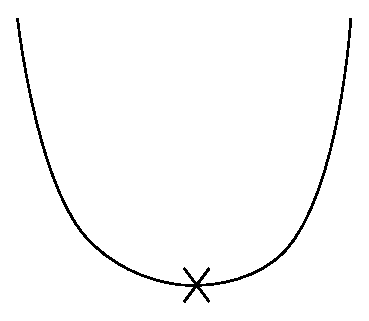
\includegraphics[scale=0.6]{img/local-min}} \\
    \centering
  \caption{Different options for when $\frac{dy}{dx}=0$.}
  \label{fig:exponent-graphs}
\end{figure}

In order to tell which of these occurs at a given point, we must look at the second derivative.

\begin{definition}
The \textbf{second derivative} of a function, written $f''(x)$ or $\frac{d^2f}{dx^2}$ is obtained by differentiating $\frac{dy}{dx}$.
\end{definition}

\begin{example}
If $$f(x)=x^3$$ then $$f'(x)=3x^2$$ and $$f''(x)=6x.$$
\end{example}

The second derivative gives that rate at which the gradient is changing.
If the gradient is increasing at a turning point, then the point is a minimum.
Similarly, if the gradient is decreasing at a turning point, then the point is a maximum.
If the second derivative is 0 at the turning point, we need more information.

\begin{in_a_box}
\begin{figure}[H]
    \subfigure[Local maximum $$f'(x)=0$$ $$f''(x)<0$$]{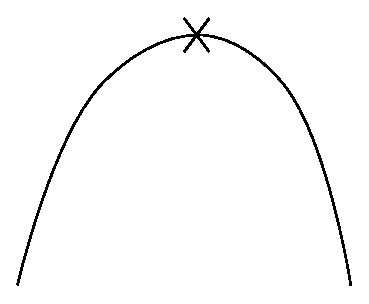
\includegraphics[scale=0.6]{img/local-max}}
    \hspace{1cm}
    \subfigure[Local minimum $$f'(x)=0$$ $$f''(x)>0$$]{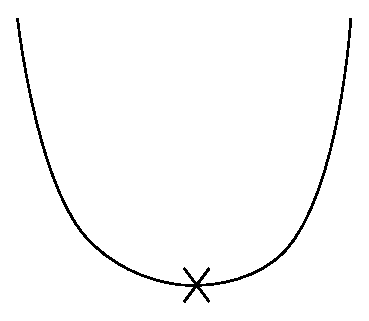
\includegraphics[scale=0.6]{img/local-min}}
    \hspace{1cm}
    \subfigure[Need more information $$f'(x)=0$$ $$f''(x)=0$$]{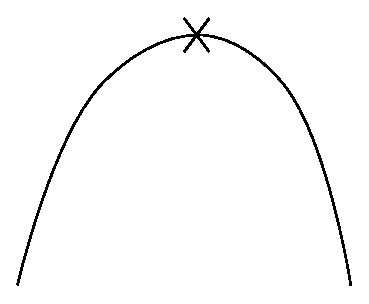
\includegraphics[scale=0.25]{img/local-max}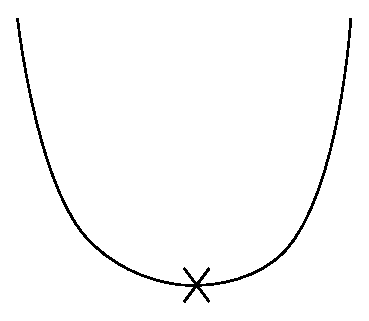
\includegraphics[scale=0.25]{img/local-min}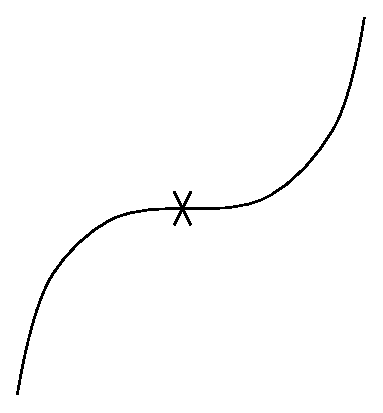
\includegraphics[scale=0.25]{img/local-inflection}} \\
    \centering
  \caption{Different options for when $\frac{dy}{dx}=0$.}
  \label{fig:exponent-graphs}
\end{figure}

\end{in_a_box}

\begin{example}
Let $f(x)=x^2$.

$f'(x)=2x$, so $f$ has a turning point at $x=0$.

$f''(x)=2$, so $f''(0)>0$. Therefore the turning point is a minimum
\end{example}
\begin{example}
Let $f(x)=x^3$.

$f'(x)=3x^2$, so $f$ has a turning point at $x=0$.

$f''(x)=6x$, so $f''(0)=0$. We need more information to decide what happens at this point.

In this case, at $x=0$ there is a point of inflection.
\end{example}
\begin{example}
Let $f(x)=x^4$.

$f'(x)=4x^3$, so $f$ has a turning point at $x=0$.

$f''(x)=12x^2$, so $f''(0)=0$. We need more information to decide what happens at this point.

In this case, at $x=0$ there is a minimum.
\end{example}
